\documentclass{article}

\usepackage{graphicx}

% to set a divider
\newcommand{\divider}{\noindent\makebox[\linewidth]{\rule{\columnwidth}{0.4pt}}}

% to count questions
\newcounter{QuestionNumber}
\newcommand{\question}{\stepcounter{QuestionNumber} {\bf Question: \arabic{QuestionNumber}}}


\begin{document}
	

\section{Quiz: latex-calculated}

\subsection{square}
Calcolare l'area del quadrato rappresentato in figura usando il valore del diametro $d$.

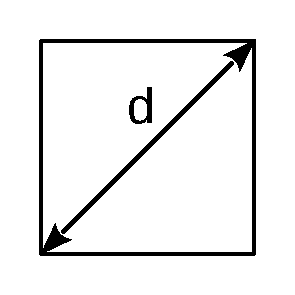
\includegraphics[width=0.3\columnwidth]{./img/square}

Dati: d = \{d\} m

\begin{itemize}
	\item answer: \texttt{pow((\{d\} / sqrt(2)),2)}
	\item fraction: 100
	\item tolerance: 0.08
	\item tolerancetype: relative % relative/nominal/geometric
	\item correctanswerformat: decimal % decimal/significant figures
	\item correctanswerlength: 2
\end{itemize}

\begin{description}
	\item[param:] d
	\begin{description}
		\item[database] private  % private/shared
		\item[minimum] 1
		\item[maximum] 10
		\item[decimals] 2
		\item[value] 2
		\item[distribution] uniform   % uniform/loguniform
	\end{description}
\end{description}


\subsection{triangle}
Calcolare l'ipotenusa $c$.


\includegraphics[width=0.3\columnwidth]{./img/triangle}

Dati: a = \{a\} m, b = \{b\} m

\begin{itemize}
	\item answer: \texttt{sqrt(pow(\{a\},2) + pow(\{b\},2))}
	\item fraction: 100
	\item tolerance: 0.1
	\item tolerancetype: relative % relative/nominal/geometric
	\item correctanswerformat: decimal % decimal/significant figures
	\item correctanswerlength: 2
\end{itemize}

\begin{description}
	\item[param:] a
	\begin{description}
		\item[database] private  % private/shared
		\item[minimum] 1
		\item[maximum] 5
		\item[decimals] 0
		\item[value] 3
		\item[distribution] uniform   % uniform/loguniform
	\end{description}
	\item[param:] b
	\begin{description}
		\item[database] private  % private/shared
		\item[minimum] 6
		\item[maximum] 10
		\item[decimals] 0
		\item[value] 8
		\item[distribution] uniform   % uniform/loguniform
    \end{description}
\end{description}


\end{document}